\section{Area-Loss Estimate}
\label{sec:strategy3-summary}

Let
\[
 A_\triangle=\frac{\sqrt3}{4}
\]
be the area of a unit equilateral triangle.  For $a,b\in[0,1]$, let
$\mathcal T(a,b)$ be the family of closed unit equilateral triangles
containing
\[
 V_0,
 \qquad
 V_0+a(V_5-V_0),
 \qquad
 V_0+b(V_1-V_0).
\]
Define the least normalized area forced outside the hexagon by
\[
 \mathcal L(a,b)=
 \inf_{T\in\mathcal T(a,b)}
 \frac{\operatorname{area}(T\setminus H)}{A_\triangle}.
\]
By reflection in the radial axis,
\[
 \mathcal L(a,b)=\mathcal L(b,a).
\]
The normalized area of $H$ is six.

\begin{figure}[H]
\centering
\begin{minipage}[b]{.48\textwidth}
\centering
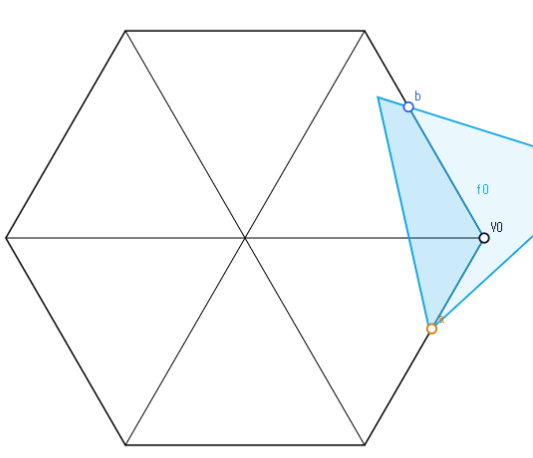
\includegraphics[width=\linewidth]{figures/strategy3_local_area_loss.png}
\par\smallskip
\footnotesize (a) local loss
\end{minipage}\hfill
\begin{minipage}[b]{.48\textwidth}
\centering
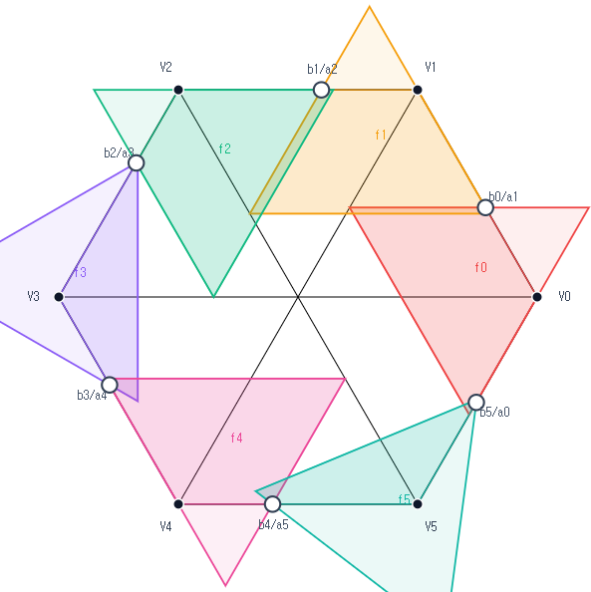
\includegraphics[width=\linewidth]{figures/strategy3_global_area_loss.png}
\par\smallskip
\footnotesize (b) cyclic sum
\end{minipage}
\caption{Local normalized area loss and its cyclic sum over the six vertex
triangles.}
\label{fig:body-area-loss}
\end{figure}

\begin{proposition}[Local area-loss bounds]
\label{prop:body-area-register}
For every feasible selected reach pair,
\[
 \mathcal L(a,b)\ge\min\{a,b\}^2.
\]
If $a+b>1$, then
\[
 \mathcal L(a,b)\ge\max\{a,b\}^2.
\]
For a $\Tlike$ triangle, $a+b\le1$, and for $0\le\mu\le1/2$,
\[
 a,b\ge\mu
 \quad\Longrightarrow\quad
 \mathcal L(a,b)\ge2\mu-4\mu^2.
\]
\end{proposition}

\begin{proof}
These are Theorems~\ref{thm:local-square-loss} and
\ref{thm:t3-direct-loss}.
\end{proof}

Assume the six vertex triangles cover $\partial H$.  Choose strict handoff
parameters
\[
 \xi_i\in(1-A_{i+1},B_i)
\]
and set
\[
 (a_i,b_i)=(1-\xi_{i-1},\xi_i).
\]
Call index $i$ an \emph{ascent} when
\[
 \xi_{i-1}<\xi_i.
\]
Equivalently, the selected reaches of $T_i$ satisfy $a_i+b_i>1$.

\begin{lemma}[Ascent structure]
\label{lem:body-ascent-structure}
The handoff parameters may be chosen so that:
\begin{enumerate}
\item if at least two vertex triangles are supercritical, at least two indices
are ascents;
\item if exactly one vertex triangle, indexed by $p$, is supercritical, then
$p$ is the unique ascent, $\xi_{p-1}$ is the global minimum, and $\xi_p$ is
the global maximum.
\end{enumerate}
\end{lemma}

\begin{proof}
The first assertion is Proposition~\ref{prop:strict-handoffs}.  In the second
case every nonsupercritical index is a strict descent, and the same proposition
makes $p$ the unique ascent.  Traversing the remaining five indices therefore
gives the stated minimum and maximum.
\end{proof}

Put
\[
 \mu=\min_i\xi_i,
 \qquad
 M=\max_i\xi_i.
\]
Reflection and reversal replace $\xi_i$ by $1-\xi_{-i-1}$, preserve every
local loss, and interchange $\mu$ with $1-M$.  Hence we may assume
\[
 \mu\le1-M.
\]
Then every $\xi_i$ and $1-\xi_i$ is at least $\mu$.

Suppose first that there are at least two supercritical vertex triangles.  By
Lemma~\ref{lem:body-ascent-structure}, the handoff parameters may be chosen
with at least two ascents.  At the first ascent leaving a cyclic block on which
$\xi_i=\mu$, the corresponding triangle has one selected reach equal to
$1-\mu$ and therefore loses at least $(1-\mu)^2$.  At a second ascent, one of
the two selected reaches is strictly larger than $1/2$, so its loss is
strictly larger than $1/4$.  Each of the remaining four triangles loses at
least $\mu^2$.  Thus the total normalized loss is strictly larger than
\[
 4\mu^2+(1-\mu)^2+\frac14
 =5\left(\mu-\frac15\right)^2+\frac{21}{20}>1.
\]

If there is exactly one supercritical vertex triangle,
Lemma~\ref{lem:body-ascent-structure} shows that its unique ascent runs from
the global minimum to the global maximum.  A distinct $\Tlike$ triangle loses
at least $2\mu-4\mu^2$, the supercritical triangle loses at least
$(1-\mu)^2$, and the other four triangles lose at least $\mu^2$ each.  The
sum is
\[
 (1-\mu)^2+(2\mu-4\mu^2)+4\mu^2=1+\mu^2>1.
\]
In either case the six vertex triangles have total area inside $H$ strictly
below five; the center triangle has area one.

\begin{proposition}[Cases excluded by area loss]
\label{prop:body-area-branches}
The area-loss argument excludes:
\begin{enumerate}
\item $T_C$ is $\CEzero$ and $N_+\ge2$, for arbitrary vertex types;
\item $T_C$ is $\CEzero$, $N_+=1$, no triangle is $\Vdone$ or $\Vdtwo$, and
at least one triangle is $\Tlike$.
\end{enumerate}
\end{proposition}

\begin{proof}
For CE0 the six vertex triangles cover $\partial H$, so
Proposition~\ref{prop:body-structural-reduction} supplies strict handoff
parameters preserving the maximal-reach supercritical pattern.  The two sums
above apply.  The detailed local calculations are in
Appendix~\ref{sec:area}.
\end{proof}
